% Figure: Autonomic Baroreflex and Orthostatic Intolerance Model
% Control-systems diagram for Chapter 29 (Neuroendocrine Models)

\begin{figure}[htbp]
\centering
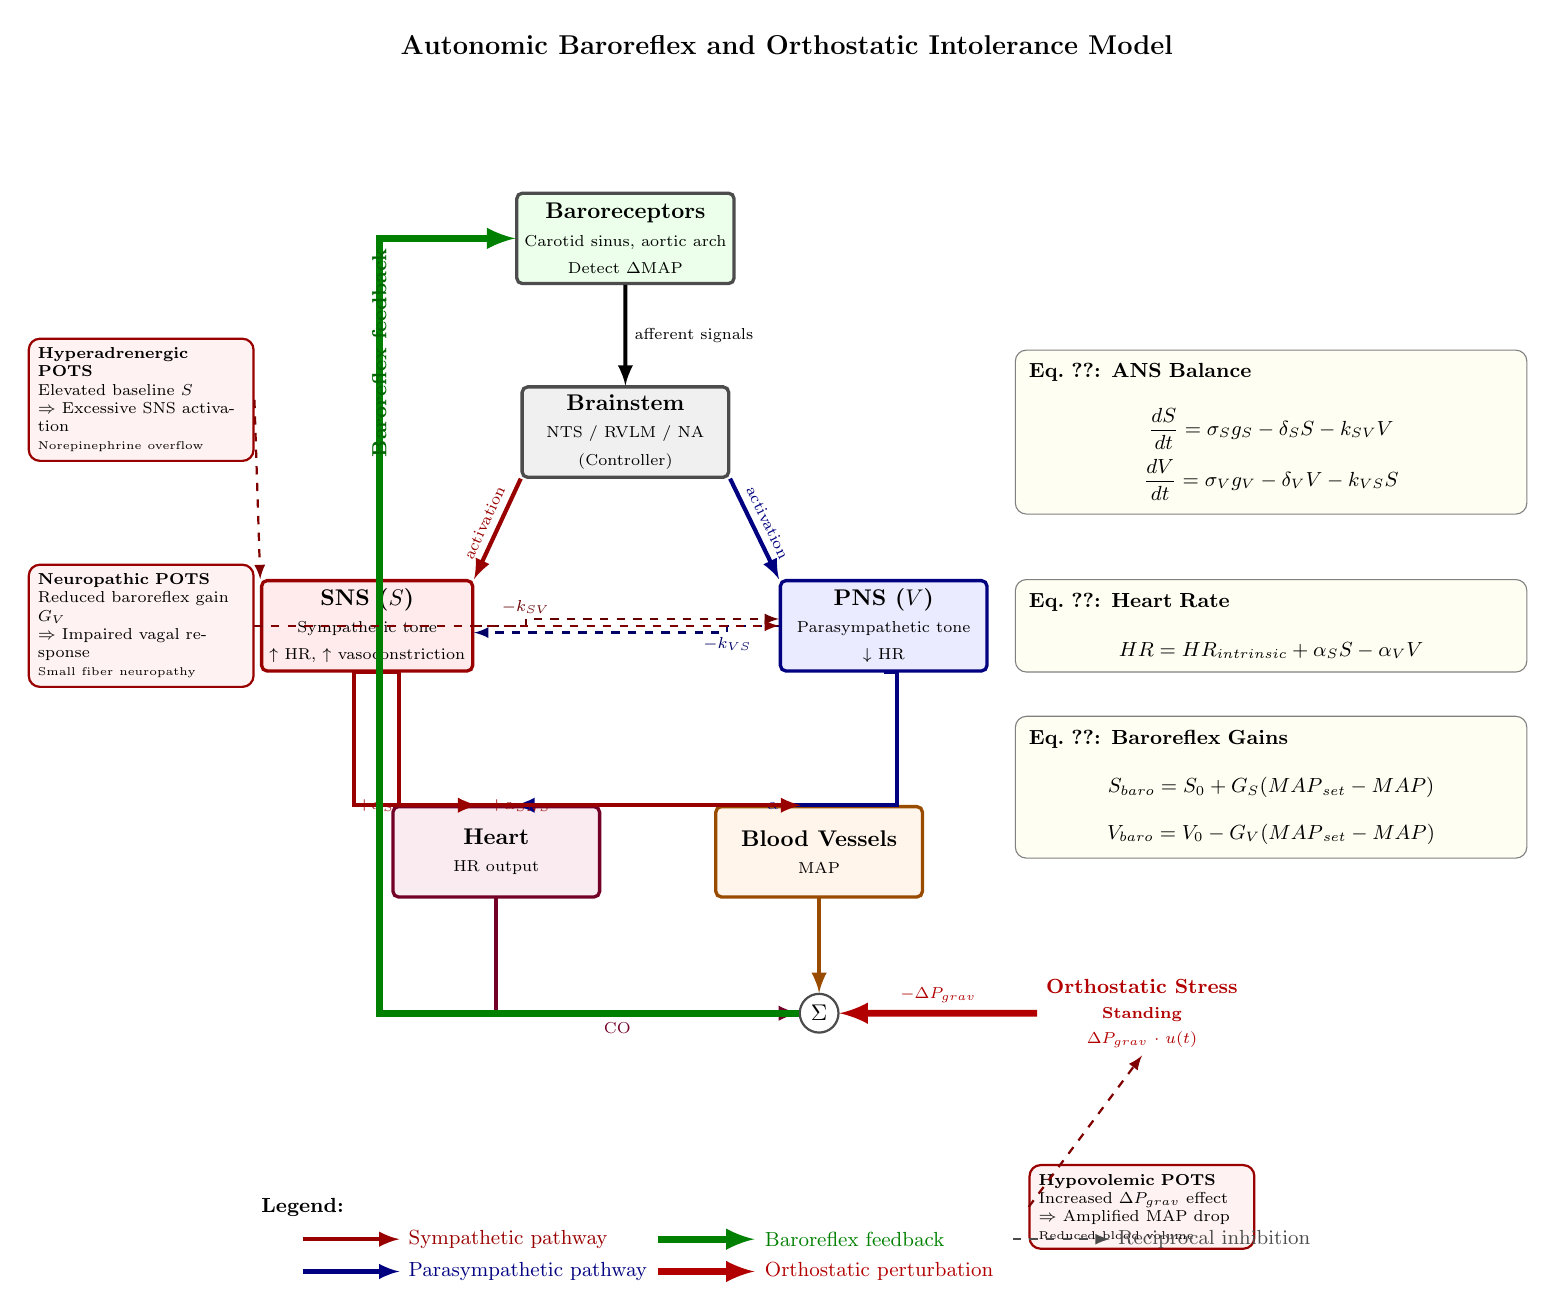
\begin{tikzpicture}[
    scale=0.82, every node/.style={scale=0.82},
    % Component styles (control-system convention)
    sensor/.style={draw=black!70, very thick, rounded corners=2pt, minimum width=3.2cm, minimum height=1.4cm, align=center, fill=green!8},
    controller/.style={draw=black!70, very thick, rounded corners=2pt, minimum width=3.2cm, minimum height=1.4cm, align=center, fill=gray!12},
    effector/.style={draw=black!70, very thick, rounded corners=2pt, minimum width=3.2cm, minimum height=1.4cm, align=center},
    sns-style/.style={effector, draw=red!60!black, fill=red!8},
    pns-style/.style={effector, draw=blue!50!black, fill=blue!8},
    heart-style/.style={effector, draw=purple!60!black, fill=purple!8},
    map-style/.style={effector, draw=orange!60!black, fill=orange!8},
    % Junction point (summing junction)
    junction/.style={circle, draw=black!70, thick, minimum size=0.6cm, inner sep=0pt, fill=white},
    % Arrow styles
    main-arrow/.style={-latex, very thick, line width=1.5pt},
    feedback-arrow/.style={-latex, ultra thick, line width=2.5pt, green!50!black},
    perturb-arrow/.style={-latex, ultra thick, line width=2.5pt, red!70!black},
    % Annotation boxes (POTS subtypes)
    pots-box/.style={draw=red!60!black, fill=red!5, rounded corners, font=\scriptsize, text width=3.2cm, align=left, inner sep=4pt, thick},
    % Equation box
    eq-box/.style={draw=black!50, fill=yellow!5, rounded corners, font=\small, inner sep=6pt, align=left},
]

% === TITLE ===
\node[font=\large\bfseries] at (2.5, 10) {Autonomic Baroreflex and Orthostatic Intolerance Model};

% === MAIN LOOP NODES ===

% Baroreceptors (top, sensor)
\node[sensor] (baro) at (0, 7) {\textbf{Baroreceptors}\\{\scriptsize Carotid sinus, aortic arch}\\{\scriptsize Detect $\Delta$MAP}};

% Brainstem (controller)
\node[controller] (brain) at (0, 4) {\textbf{Brainstem}\\{\scriptsize NTS / RVLM / NA}\\{\scriptsize (Controller)}};

% SNS (left branch)
\node[sns-style] (sns) at (-4, 1) {\textbf{SNS ($S$)}\\{\scriptsize Sympathetic tone}\\{\scriptsize $\uparrow$ HR, $\uparrow$ vasoconstriction}};

% PNS (right branch)
\node[pns-style] (pns) at (4, 1) {\textbf{PNS ($V$)}\\{\scriptsize Parasympathetic tone}\\{\scriptsize $\downarrow$ HR}};

% Heart (effector, center-left below)
\node[heart-style] (heart) at (-2, -2.5) {\textbf{Heart}\\{\scriptsize HR output}};

% MAP (effector, center-right below)
\node[map-style] (map) at (3, -2.5) {\textbf{Blood Vessels}\\{\scriptsize MAP}};

% Summing junction before MAP
\node[junction] (sum) at (3, -5) {$\Sigma$};

% === MAIN FLOW ARROWS ===

% Baro -> Brainstem
\draw[main-arrow] (baro) -- (brain) node[midway, right, font=\scriptsize] {afferent signals};

% Brainstem -> SNS (excitatory)
\draw[main-arrow, red!60!black] (brain.south west) -- (sns.north east) node[midway, above, font=\scriptsize, sloped] {activation};

% Brainstem -> PNS (excitatory)
\draw[main-arrow, blue!50!black] (brain.south east) -- (pns.north west) node[midway, above, font=\scriptsize, sloped] {activation};

% Reciprocal inhibition between SNS and PNS
\draw[-latex, thick, dashed, red!40!black] (sns.east) -- ++(0.8, 0) |- ([yshift=3pt]pns.west) node[pos=0.25, above, font=\scriptsize] {$-k_{SV}$};
\draw[-latex, thick, dashed, blue!40!black] (pns.west) -- ++(-0.8, 0) |- ([yshift=-3pt]sns.east) node[pos=0.25, below, font=\scriptsize] {$-k_{VS}$};

% SNS -> Heart
\draw[main-arrow, red!60!black] (sns.south) -- ++(-0.2,0) |- ([xshift=-8pt]heart.north) node[pos=0.7, left, font=\scriptsize] {$+\alpha_S$};

% PNS -> Heart
\draw[main-arrow, blue!50!black] (pns.south) -- ++(0.2,0) |- ([xshift=8pt]heart.north) node[pos=0.7, right, font=\scriptsize] {$-\alpha_V$};

% SNS -> Blood Vessels (vasoconstriction)
\draw[main-arrow, red!60!black] (sns.south) -- ++(0.5, 0) |- ([xshift=-8pt]map.north) node[pos=0.7, left, font=\scriptsize] {$+\alpha_{\text{SNS}}$};

% Heart -> MAP (cardiac output contributes to MAP)
\draw[main-arrow, purple!60!black] (heart.south) |- (sum.west) node[pos=0.7, below, font=\scriptsize] {CO};

% MAP output from summing junction
\draw[main-arrow, orange!60!black] (map.south) -- (sum.north);

% === FEEDBACK LOOP (Baroreflex) ===
% MAP feeds back to baroreceptors (closing the loop)
\draw[feedback-arrow] (sum.west) -- ++(-6.5, 0) |- (baro.west)
    node[pos=0.5, left, font=\small\bfseries, text=green!40!black, rotate=90] {Baroreflex feedback};

% === ORTHOSTATIC PERTURBATION ===
\node[font=\small\bfseries, red!70!black, text width=3cm, align=center] (stand) at (8, -5) {\textbf{Orthostatic Stress}\\{\scriptsize Standing}\\{\scriptsize $\Delta P_{\text{grav}} \cdot u(t)$}};
\draw[perturb-arrow] (stand) -- (sum) node[midway, above, font=\scriptsize] {$-\Delta P_{\text{grav}}$};

% === EQUATION BOXES ===

% ANS balance equation
\node[eq-box, text width=7.5cm] at (10, 4) {
    \textbf{Eq.~\ref{eq:ans-balance}: ANS Balance}
    \vspace{2pt}
    \[
    \frac{dS}{dt} = \sigma_S g_S - \delta_S S - k_{SV} V
    \]
    \vspace{-10pt}
    \[
    \frac{dV}{dt} = \sigma_V g_V - \delta_V V - k_{VS} S
    \]
};

% HR equation
\node[eq-box, text width=7.5cm] at (10, 1) {
    \textbf{Eq.~\ref{eq:heart-rate}: Heart Rate}
    \vspace{2pt}
    \[
    \text{HR} = \text{HR}_{\text{intrinsic}} + \alpha_S S - \alpha_V V
    \]
};

% Baroreflex gains
\node[eq-box, text width=7.5cm] at (10, -1.5) {
    \textbf{Eq.~\ref{eq:baroreflex}: Baroreflex Gains}
    \vspace{2pt}
    \[
    S_{\text{baro}} = S_0 + G_S(\text{MAP}_{\text{set}} - \text{MAP})
    \]
    \vspace{-10pt}
    \[
    V_{\text{baro}} = V_0 - G_V(\text{MAP}_{\text{set}} - \text{MAP})
    \]
};

% === POTS SUBTYPE ANNOTATIONS ===

% Neuropathic POTS
\node[pots-box] (pots1) at (-7.5, 1) {
    \textbf{Neuropathic POTS}\\
    Reduced baroreflex gain $G_V$\\
    $\Rightarrow$ Impaired vagal response\\
    {\tiny Small fiber neuropathy}
};
\draw[-latex, thick, red!50!black, dashed] (pots1.east) -- (pns.west);

% Hyperadrenergic POTS
\node[pots-box] (pots2) at (-7.5, 4.5) {
    \textbf{Hyperadrenergic POTS}\\
    Elevated baseline $S$\\
    $\Rightarrow$ Excessive SNS activation\\
    {\tiny Norepinephrine overflow}
};
\draw[-latex, thick, red!50!black, dashed] (pots2.east) -- (sns.north west);

% Hypovolemic POTS
\node[pots-box] (pots3) at (8, -8) {
    \textbf{Hypovolemic POTS}\\
    Increased $\Delta P_{\text{grav}}$ effect\\
    $\Rightarrow$ Amplified MAP drop\\
    {\tiny Reduced blood volume}
};
\draw[-latex, thick, red!50!black, dashed] (pots3.west) -- (stand.south);

% === LEGEND ===
\begin{scope}[yshift=-8.5cm, xshift=-5cm]
    \node[font=\small\bfseries] at (0, 0.5) {Legend:};
    \draw[main-arrow, red!60!black] (0, 0) -- (1.5, 0) node[right, font=\small] {Sympathetic pathway};
    \draw[main-arrow, blue!50!black] (0, -0.5) -- (1.5, -0.5) node[right, font=\small] {Parasympathetic pathway};
    \draw[feedback-arrow] (5.5, 0) -- (7, 0) node[right, font=\small] {Baroreflex feedback};
    \draw[perturb-arrow] (5.5, -0.5) -- (7, -0.5) node[right, font=\small] {Orthostatic perturbation};
    \draw[-latex, thick, dashed, gray!60!black] (11, 0) -- (12.5, 0) node[right, font=\small] {Reciprocal inhibition};
\end{scope}

\end{tikzpicture}
\caption{Baroreflex control loop model (Equations~\ref{eq:ans-balance}--\ref{eq:baroreflex}). Baroreceptors detect MAP changes and modulate sympathetic ($S$) and parasympathetic ($V$) tone to maintain cardiovascular homeostasis. Orthostatic stress (standing) reduces MAP, triggering compensatory responses. Three ME/CFS-associated POTS subtypes correspond to distinct parameter modifications in the model.}
\label{fig:baroreflex-model}
\end{figure}
